\chapter{Experiments}
\label{chap:Experiments}
This chapter describes the different experiments we ran as well as their respective results. It is heavily focusing on the task at hand, which is to \emph{predict the diagnosed top 50 most frequent ICD9 codes at discharge in a multi-class multi-classification fashion}. \\

The first section describes the setup in which the experiments are run, the optimizer as well as the hardware setting. Following to this, we get to the core of the chapter and explain our experiments we ran while providing the quantitative results on different metrics. Finally, from these experiments we conclude the chapter with a hyper-parameter tuning section detailing how we picked the deep learning hyper-parameters.

\section{Setup}
\label{sec:Setup}
All the experiments and training sessions were run on two \textbf{Tesla P100} with 16 GB of memory. The CPU was an \textbf{Intel Xeon Gold 5120 CPU @ 2.20 GHz}, with \textbf{56 cores}, while we had access to \textbf{187 GB of RAM} on the machine. On top of that, the different scripts and models have been built on \textit{Python 3.6.7} and we used \textit{Pytorch 1.0.0} as our Deep Learning framework. \\

We  employ  mini-batch  stochastic gradient descent method together with the Adam optimizer~\cite{DBLP:journals/corr/KingmaB14} to  minimize  our multi-class multi-classification loss. \\

To facilitate reading and understanding, we break down the different hyper-parameters in three groups:

\begin{itemize}
 \item Knowledge Graph
 \begin{itemize}
  \item $M$: number of neighbors
  \item Characters n-grams
  \item Weighted Personalized PageRank threshold
  \item Disease - Symptom threshold
  \item Admission - Symptom threshold
  \item Admission - Disease threshold
 \end{itemize}
 \item Admission Processing
 \begin{itemize}
  \item $N$: number of chunks
  \item $K$: number of events per chunk
  \item $\tau$: chunk length
 \end{itemize}
 \item Deep Learning
 \begin{itemize}
  \item $n$: events embedding dimension (potentially different for each event type)
  \item $a$: aggregators hidden dimension (for both input entity and neighbors, potentially different for each event type)
  \item Input entity aggregator type (max, mean or sum, potentially different for each event type)
  \item Neighbor entities aggregator type (max, mean or sum)
  \item RNN: number of layers
  \item RNN: number of neurons per layer
  \item RNN: dropout between layers
  \item RNN: bidirectional or not
  \item $b$: Recurrent Neural Network output dimension
  \item Batch size
 \end{itemize}
\end{itemize}

To reduce the search space, we contrived our hyper-parameters by fixing the same embedding dimension and aggregator for all events. Finally, we also decided to tune the \emph{Knowledge Graph} and \emph{Admission Processing} hyper-parameters while tuning the \emph{Deep Learning} ones. Consequently, we also did the opposite when tuning the \emph{Knowledge Graph} and \emph{Admission Processing} hyper-parameters. \\

This way, we limit the computation time while getting a pretty good idea of the top-performing configurations and interactions between theses hyper-parameters. We suppose that scores reported for the final task on the testing set could be further improved by fine-tuning all these hyper-parameters together instead of group-by-group. \\

Finally, we decided to split the \emph{58'976} in two groups, training and testing set, using an 80\%-20\% split. We then further holdout 10\% of this training set for validation purposes (the training set is thus 72\% of the total admissions while validation represents 8\% of these). \\

As a training strategy, we monitor different metrics, as explained in the section~\ref{sec:Metrics}, at each epoch and employ an early-stopping criterion on the validation loss with a patience of 20 epochs. That is, if the validation loss does not decrease within 20 epochs, the model is saved at its best scoring epoch and the training is considered finished.

\newpage
\section{Metrics}
\label{sec:Metrics}
\paragraph{F1 Score} The $F_1$ score is a particular case of the $F_\beta$ score which blends the well-known precision and recall scores. The $F_\beta$ score is computed as follows:

\begin{equation}
 F_\beta = (1+\beta)^2 \cdot \frac{\mbox{Precision} \cdot \mbox{Recall}}{(\beta^2 \cdot \mbox{Precision}) + \mbox{Recall}}
\end{equation}

Basically, the $\beta$ parameters dictate the importance we want to give to the precision or recall. By setting $\beta=1$, we give equal importance to both of them and above formula is equivalent to computing harmonic mean between the precision and recall. Our choice of $\beta=1$ is common and usually a good trade-off when there is no obvious preference between precision and recall.

\paragraph{Area Under Receiver Operating Characteristic} Often abbreviated \textit{AUROC}, this metric is coming from the receiver operating characteristic curve that is computed using the ``True positive rate`` and ``False positive rate``. This curve is particularly interesting since it reports the ability of our classifier to discriminate between positive and negative samples when the threshold varies. \\

Generally speaking, computing the area under this ROC curve is equivalent to the probability that a classifier will rank a positive random sample \textbf{higher} than a random negative one.

\paragraph{Macro and Micro Averages} To account for the slight class imbalance depicted in the top-right figure~\ref{fig:icd9-codes}, we consider two kinds of averages over classes scores, namely \emph{macro} and \emph{micro} averages. \\

The macro average will compute the metric independently for each class and then average globally, thus treating our different ICD9 codes equally. On the other hand, the micro average will first aggregate the contributions of all classes in order to compute the average metric. \\

We decided to compute both averages for our two metrics, leading to four combinations that we report in the experiments in sections~\ref{sec:Experiments}:

\begin{itemize}
 \item Macro-F1 Score
 \item Micro-F1 Score
 \item Macro-AUROC
 \item Micro-AUROC
\end{itemize}

\newpage
\section{Deep Learning Hyper-parameter Tuning}
For the hyper-parameter tuning of deep learning parameters, we fixed the \emph{Knowledge Graph} and \emph{Admission Processing} hyper-parameters to the following values:

\begin{itemize}
 \item Knowledge Graph
 \begin{itemize}
  \item $M=10$
  \item Characters n-grams = 3 characters
  \item Weighted Personalized PageRank threshold = 0.0001
  \item Disease - Symptom threshold = 0.2
  \item Admission - Symptom threshold = 0.6
  \item Admission - Disease threshold = 0.6
 \end{itemize}
 \item Admission Processing
 \begin{itemize}
  \item $N = 200$
  \item $K = 25$
  \item $\tau = 3 \mbox{ hours}$
 \end{itemize}
\end{itemize}
\subsection{Method}

All the scores were computed on the validation set, leaving the testing one untainted to prevent overfitting. The best scoring model was chosen accordingly and in accordance to performances on the validation loss. \\

We employed a very simple \emph{random search} as a sampling strategy of the next set of hyper-parameters during the optimization. This allows for much better results than a typical grid search that has the tendency to explore only a small subset of the search space. This strategy is also proven to show very good performances when the number of \textit{trials} is limited ($\leq 100$ in our case) for a very large search space, on top of the ease of implementation compared to more advanced sampling strategies.

\subsection{Search space}
The search space in our case consisted of:

\begin{itemize}
 \item $n \in \{8, 16, 32, 64, 128\}$, same for all event types
 \item $a=64$, same for input entity, neighbors and all event types
 \item $\mbox{agg}_{\mbox{input}} \in \{\mbox{max}, \mbox{mean}, \mbox{sum}\}$, same for all event types
 \item $\mbox{agg}_{\mbox{neighbors}} \in \{\mbox{max}, \mbox{mean}, \mbox{sum}\}$, same for all event types
 \item $\mbox{RNN}_{\mbox{layers}} \in \{1, 2, 3, 4, 5\}$
 \item $\mbox{RNN}_{\mbox{neurons}} \in \{64, 128, 256, 512\}$
 \item $\mbox{RNN}_{\mbox{dropout}} \in \{0, 0.1, 0.25, 0.5\}$
 \item $\mbox{RNN}_{\mbox{bidirectional}} \in \{\mbox{True}, \mbox{False}\}$
 \item $\mbox{RNN}_{\mbox{output size}} = 64$
 \item $\mbox{Batch size} \in \{4, 8, 16, 32, 64, 128\}$
\end{itemize}
Which leaves us with a search space of $5 \times 3 \times 3 \times 5 \times 4 \times 4 \times 2 \times 6 = 43'200$ possibilities.

\subsection{Results}
\paragraph{Baseline} We obtained the following best-scoring combination of hyper-parameters for the baseline:
\begin{itemize}
 \item $n = 64$
 \item $a = 64$
 \item $\mbox{agg}_{\mbox{input}} = \mbox{mean}$
 \item $\mbox{RNN}_{\mbox{layers}} = 1$
 \item $\mbox{RNN}_{\mbox{neurons}} = 128$
 \item $\mbox{RNN}_{\mbox{dropout}} = 0.25$
 \item $\mbox{RNN}_{\mbox{bidirectional}} = \mbox{True}$
 \item $\mbox{RNN}_{\mbox{output size}} = 64$
 \item $\mbox{Batch size} = 16$
\end{itemize}
Which translates to a particularly lightweight model, indicating the tendency of the baseline to overfit rather quickly.
\paragraph{KG-RNN} We obtained the following best-scoring combination of hyper-parameters for the baseline:
\begin{itemize}
 \item $n = 16$
 \item $a = 64$
 \item $\mbox{agg}_{\mbox{input}} = \mbox{max}$
 \item $\mbox{agg}_{\mbox{neighbors}} = \mbox{mean}$
 \item $\mbox{RNN}_{\mbox{layers}} = 2$
 \item $\mbox{RNN}_{\mbox{neurons}} = 128$
 \item $\mbox{RNN}_{\mbox{dropout}} = 0.5$
 \item $\mbox{RNN}_{\mbox{bidirectional}} = \mbox{False}$
 \item $\mbox{RNN}_{\mbox{output size}} = 64$
 \item $\mbox{Batch size} = 128$
\end{itemize}
It is important to notice that this top-scoring configuration consists in using a different kind of aggregator for neighboring admissions and input events. \\

One could argue that using a \emph{max-pooling} for input events and \emph{mean-pooling} for neighbors final diagnoses make sense since we can hypothesis that most salient events are important for a single patient, while blending the final diagnoses of neighbors allows to account for their relative contributions. \\

\section{Experiments}
\label{sec:Experiments}
Each experiment is broken down in a short description of the experiment and the associated results and graphics, followed by a ``discussion`` section where we interpret the results and plots. \\

All of these are on validation set for sake of keeping the testing set untainted until the final evaluation of the task at hand, namely ICD9 code prediction. Therefore, results of the different metrics, presented in sections~\ref{sec:Metrics}, are computed on the validation set for all experiments and compared to the baseline scores on each figure. \\

For all these experiments, the base setup of hyper-parameters are the one from the previous section for the \emph{Deep Learning} group. For the two other groups, here are the default parameters we chose:

\begin{itemize}
 \item Knowledge Graph
 \begin{itemize}
  \item $M=10$
  \item Characters n-grams = 3 characters
  \item Weighted Personalized PageRank threshold = 0.0001
  \item Disease - Symptom threshold = 0.2
  \item Admission - Symptom threshold = 0.6
  \item Admission - Disease threshold = 0.6
 \end{itemize}
 \item Admission Processing
 \begin{itemize}
  \item $N = 200$
  \item $K = 25$
  \item $\tau = 3 \mbox{ hours}$
 \end{itemize}
\end{itemize}

These are the hyper-parameters to be assumed except for the varying one in each experiment, that will be reminded in the relevant subsection. It is important to bear in mind that complex interactions within hyper-parameters are not taken into account in these experiments since we tune one degree of freedom at a time. \\

It would be very interesting to run these experiments with more computational power and time to account for much more precise hyper-parameter tuning and visualize how the metrics react for possibly more complex combinations.

\newpage
\subsection{Chunk length}
In this experiment we make the number of hours per chunk vary. This means that we consider the larger time window as the current graph state. Thus, it should have an impact on the amount of information fed to \emph{KG-RNN}, especially its aggregators.

\begin{figure}[H]
 \centering
 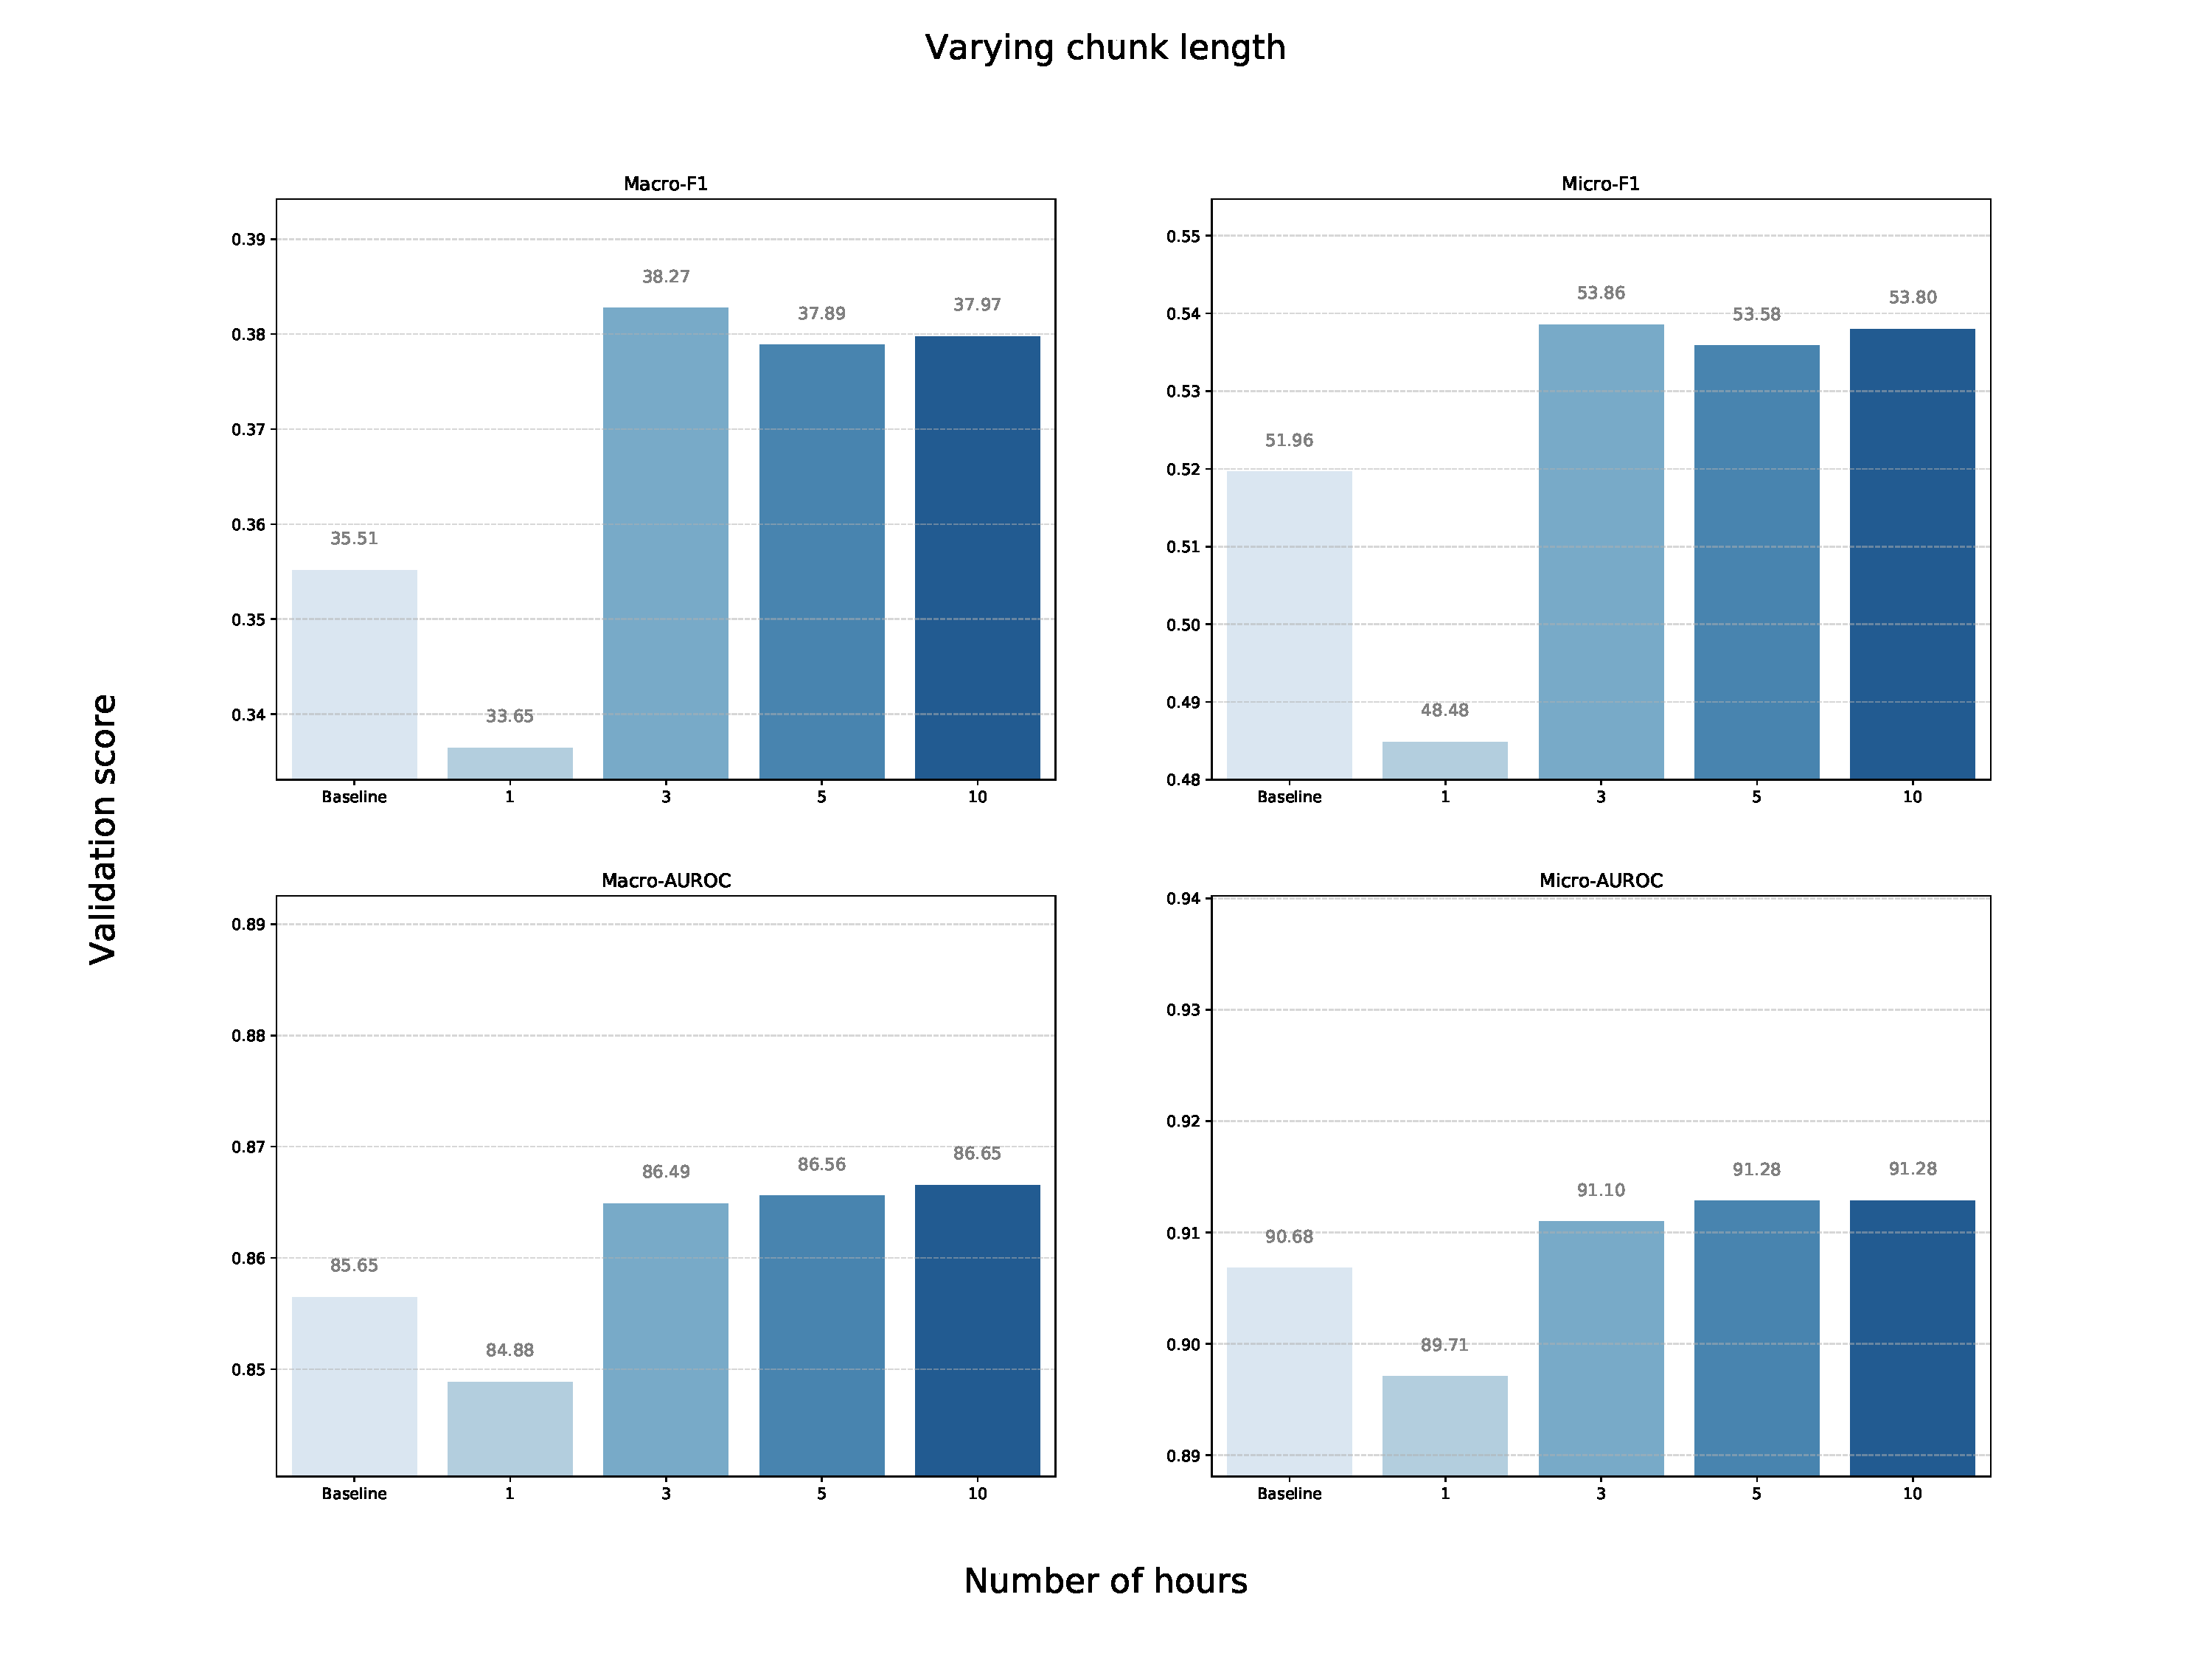
\includegraphics[width=\textwidth]{figures/exp-hours.pdf}
\end{figure}

\paragraph{Discussion} We see that the number of hours per chunk does not have a huge impact after 3 hours. However, setting the chunk length to small (i.e. 1 hour) makes the graph state probably too sparse in terms of the number of events.

\newpage
\subsection{Admission length}
This experiment makes the number of chunks per admission vary, also referred as the number of graph states. This will have the impact of increasing the size of sequences that are fed to the downstream Recurrent Neural Network and challenge its capacity to encode long-term dependencies in the input sequences.

\begin{figure}[H]
 \centering
 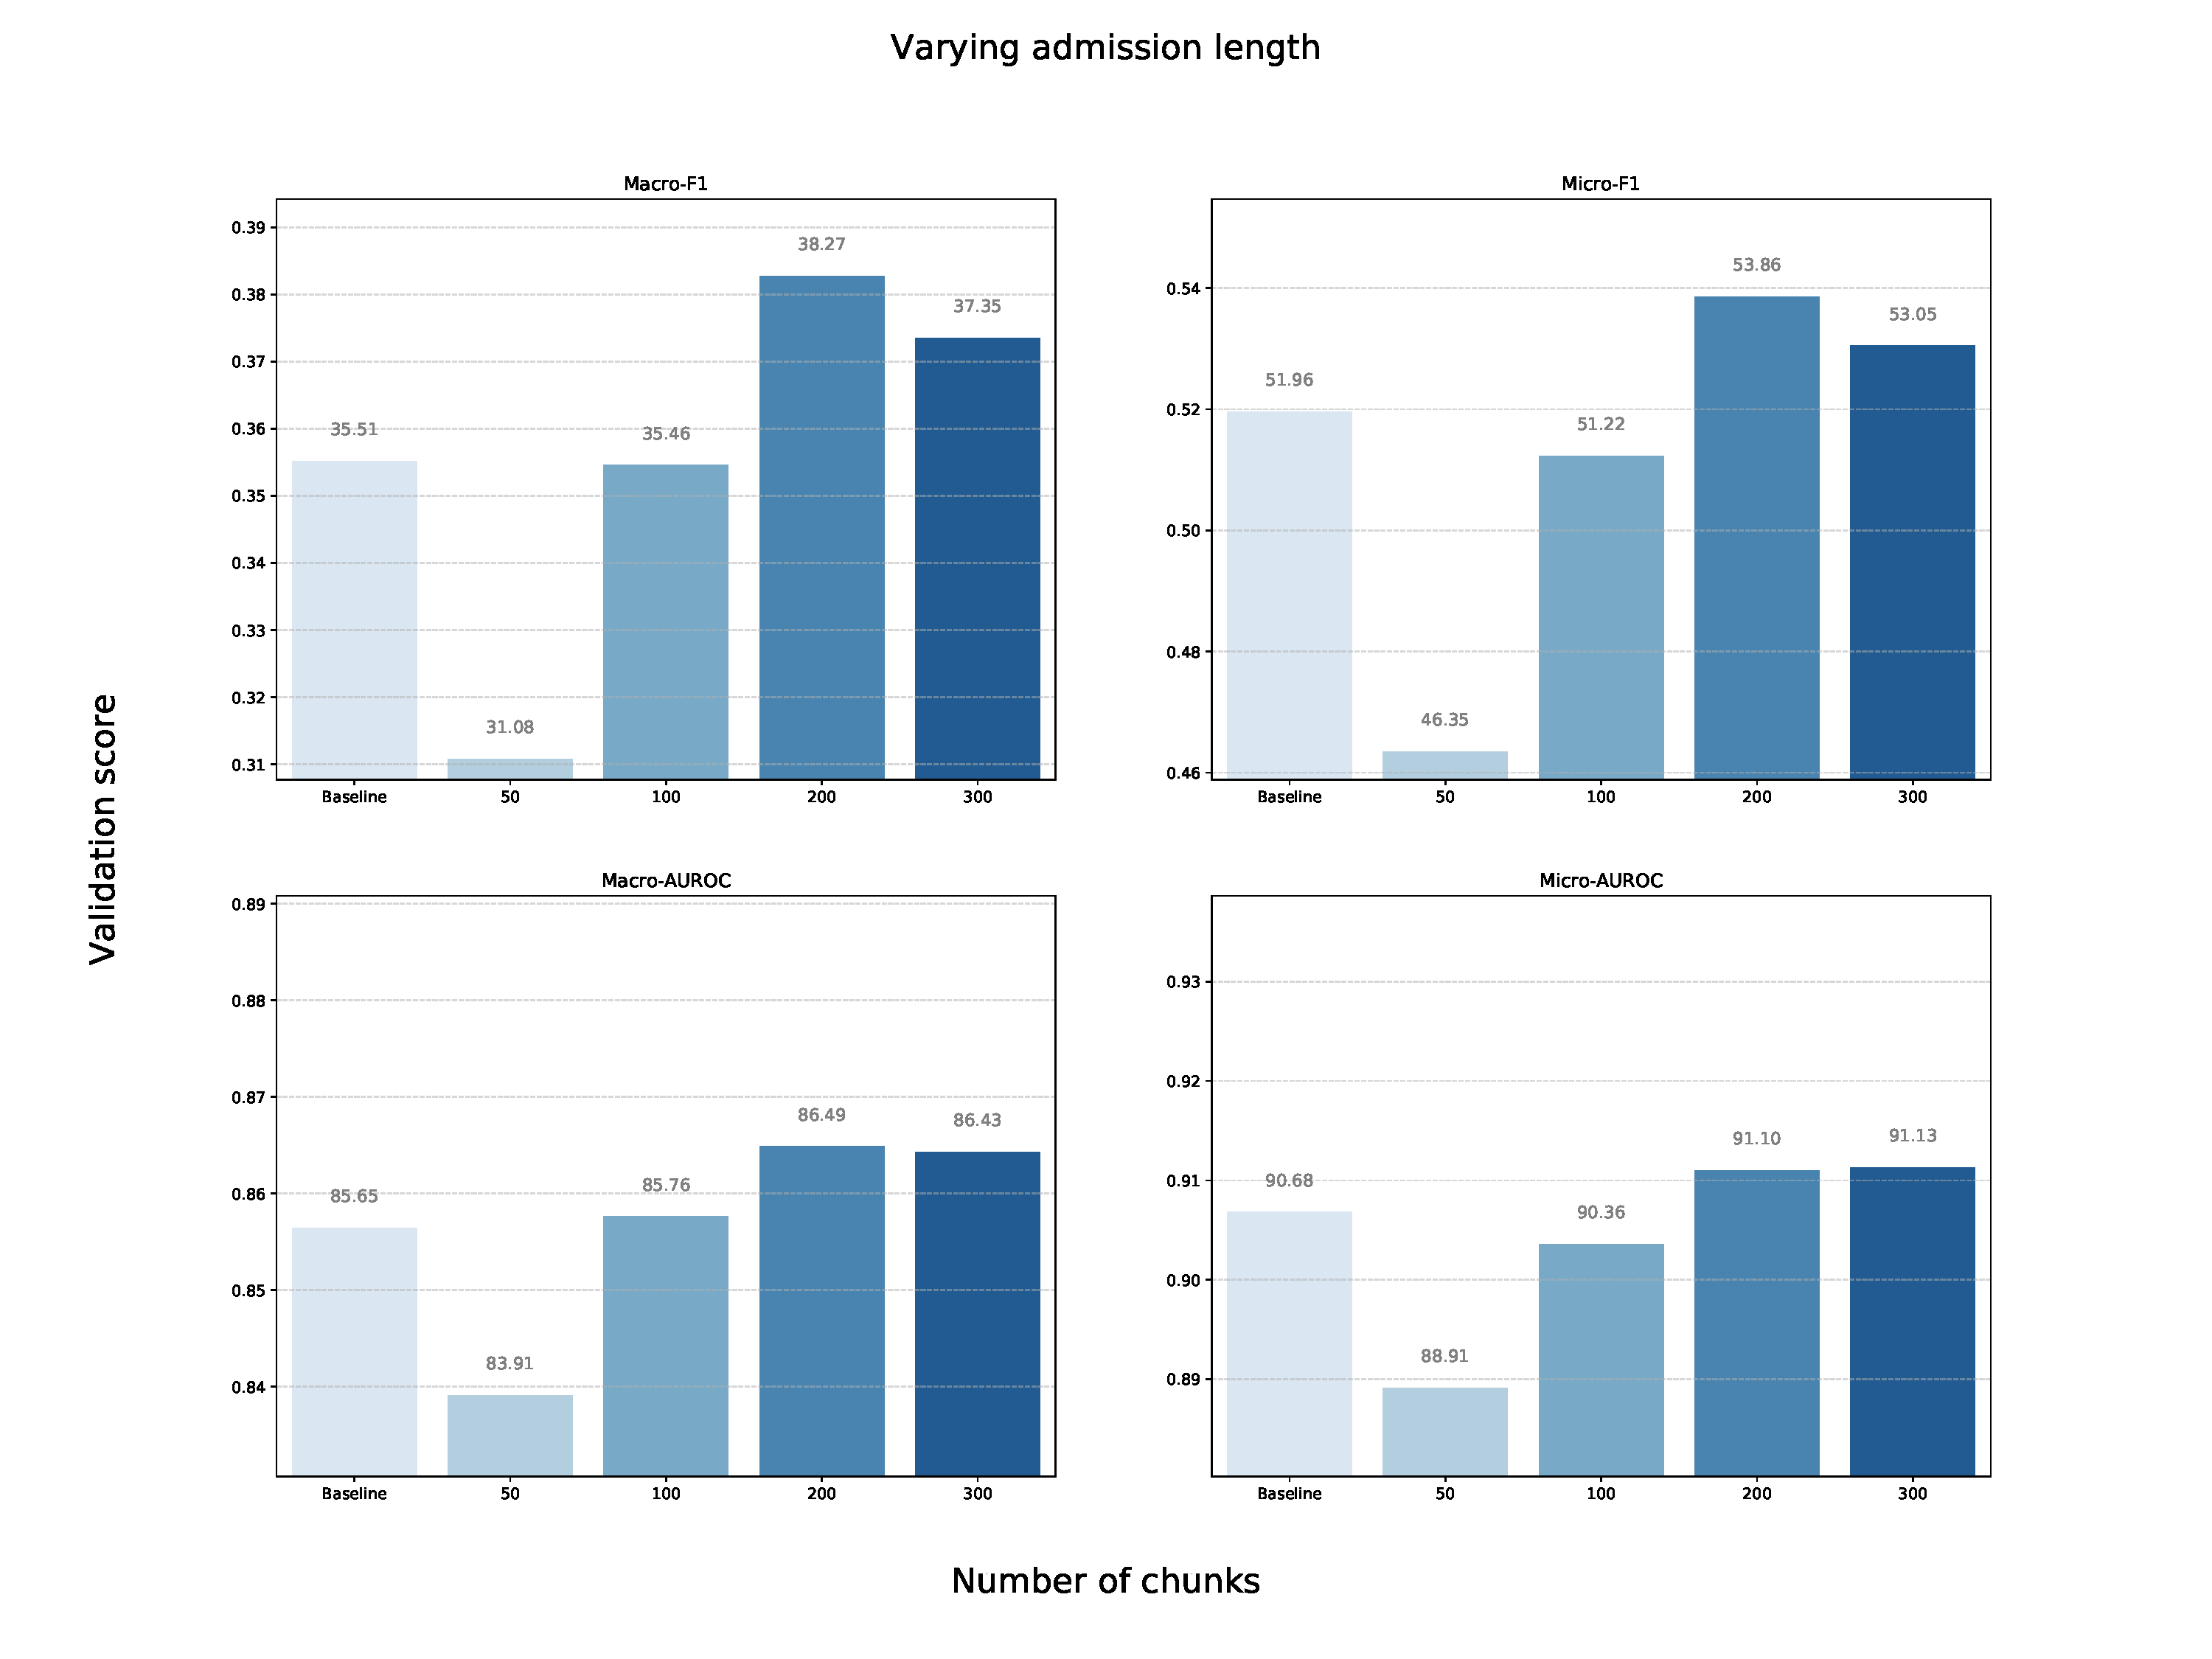
\includegraphics[width=\textwidth]{figures/exp-chunks.pdf}
\end{figure}

\paragraph{Discussion} In the above figure, we clearly see that we obtain a local optimum with an admission length of \emph{200} for the F1 score. However, the optimal value for the AUROC score is not so clear cut and further investigation would be beneficial in terms of interaction with the \textbf{chunk length}. \\

Indeed, since the total considered time for an admission is $\mbox{chunk length} \times \mbox{admission length}$, both parameters are intrinsically linked and probably heavily correlated.

\newpage
\subsection{Number of events per chunk}
For this experiment, we vary the \textit{maximum} number of events per chunk and per type. Chunks that have more than this number of events in a chunk for a given type will be randomly sampled to $K$, while other ones remain with their number of events $\leq K$.

\begin{figure}[H]
 \centering
 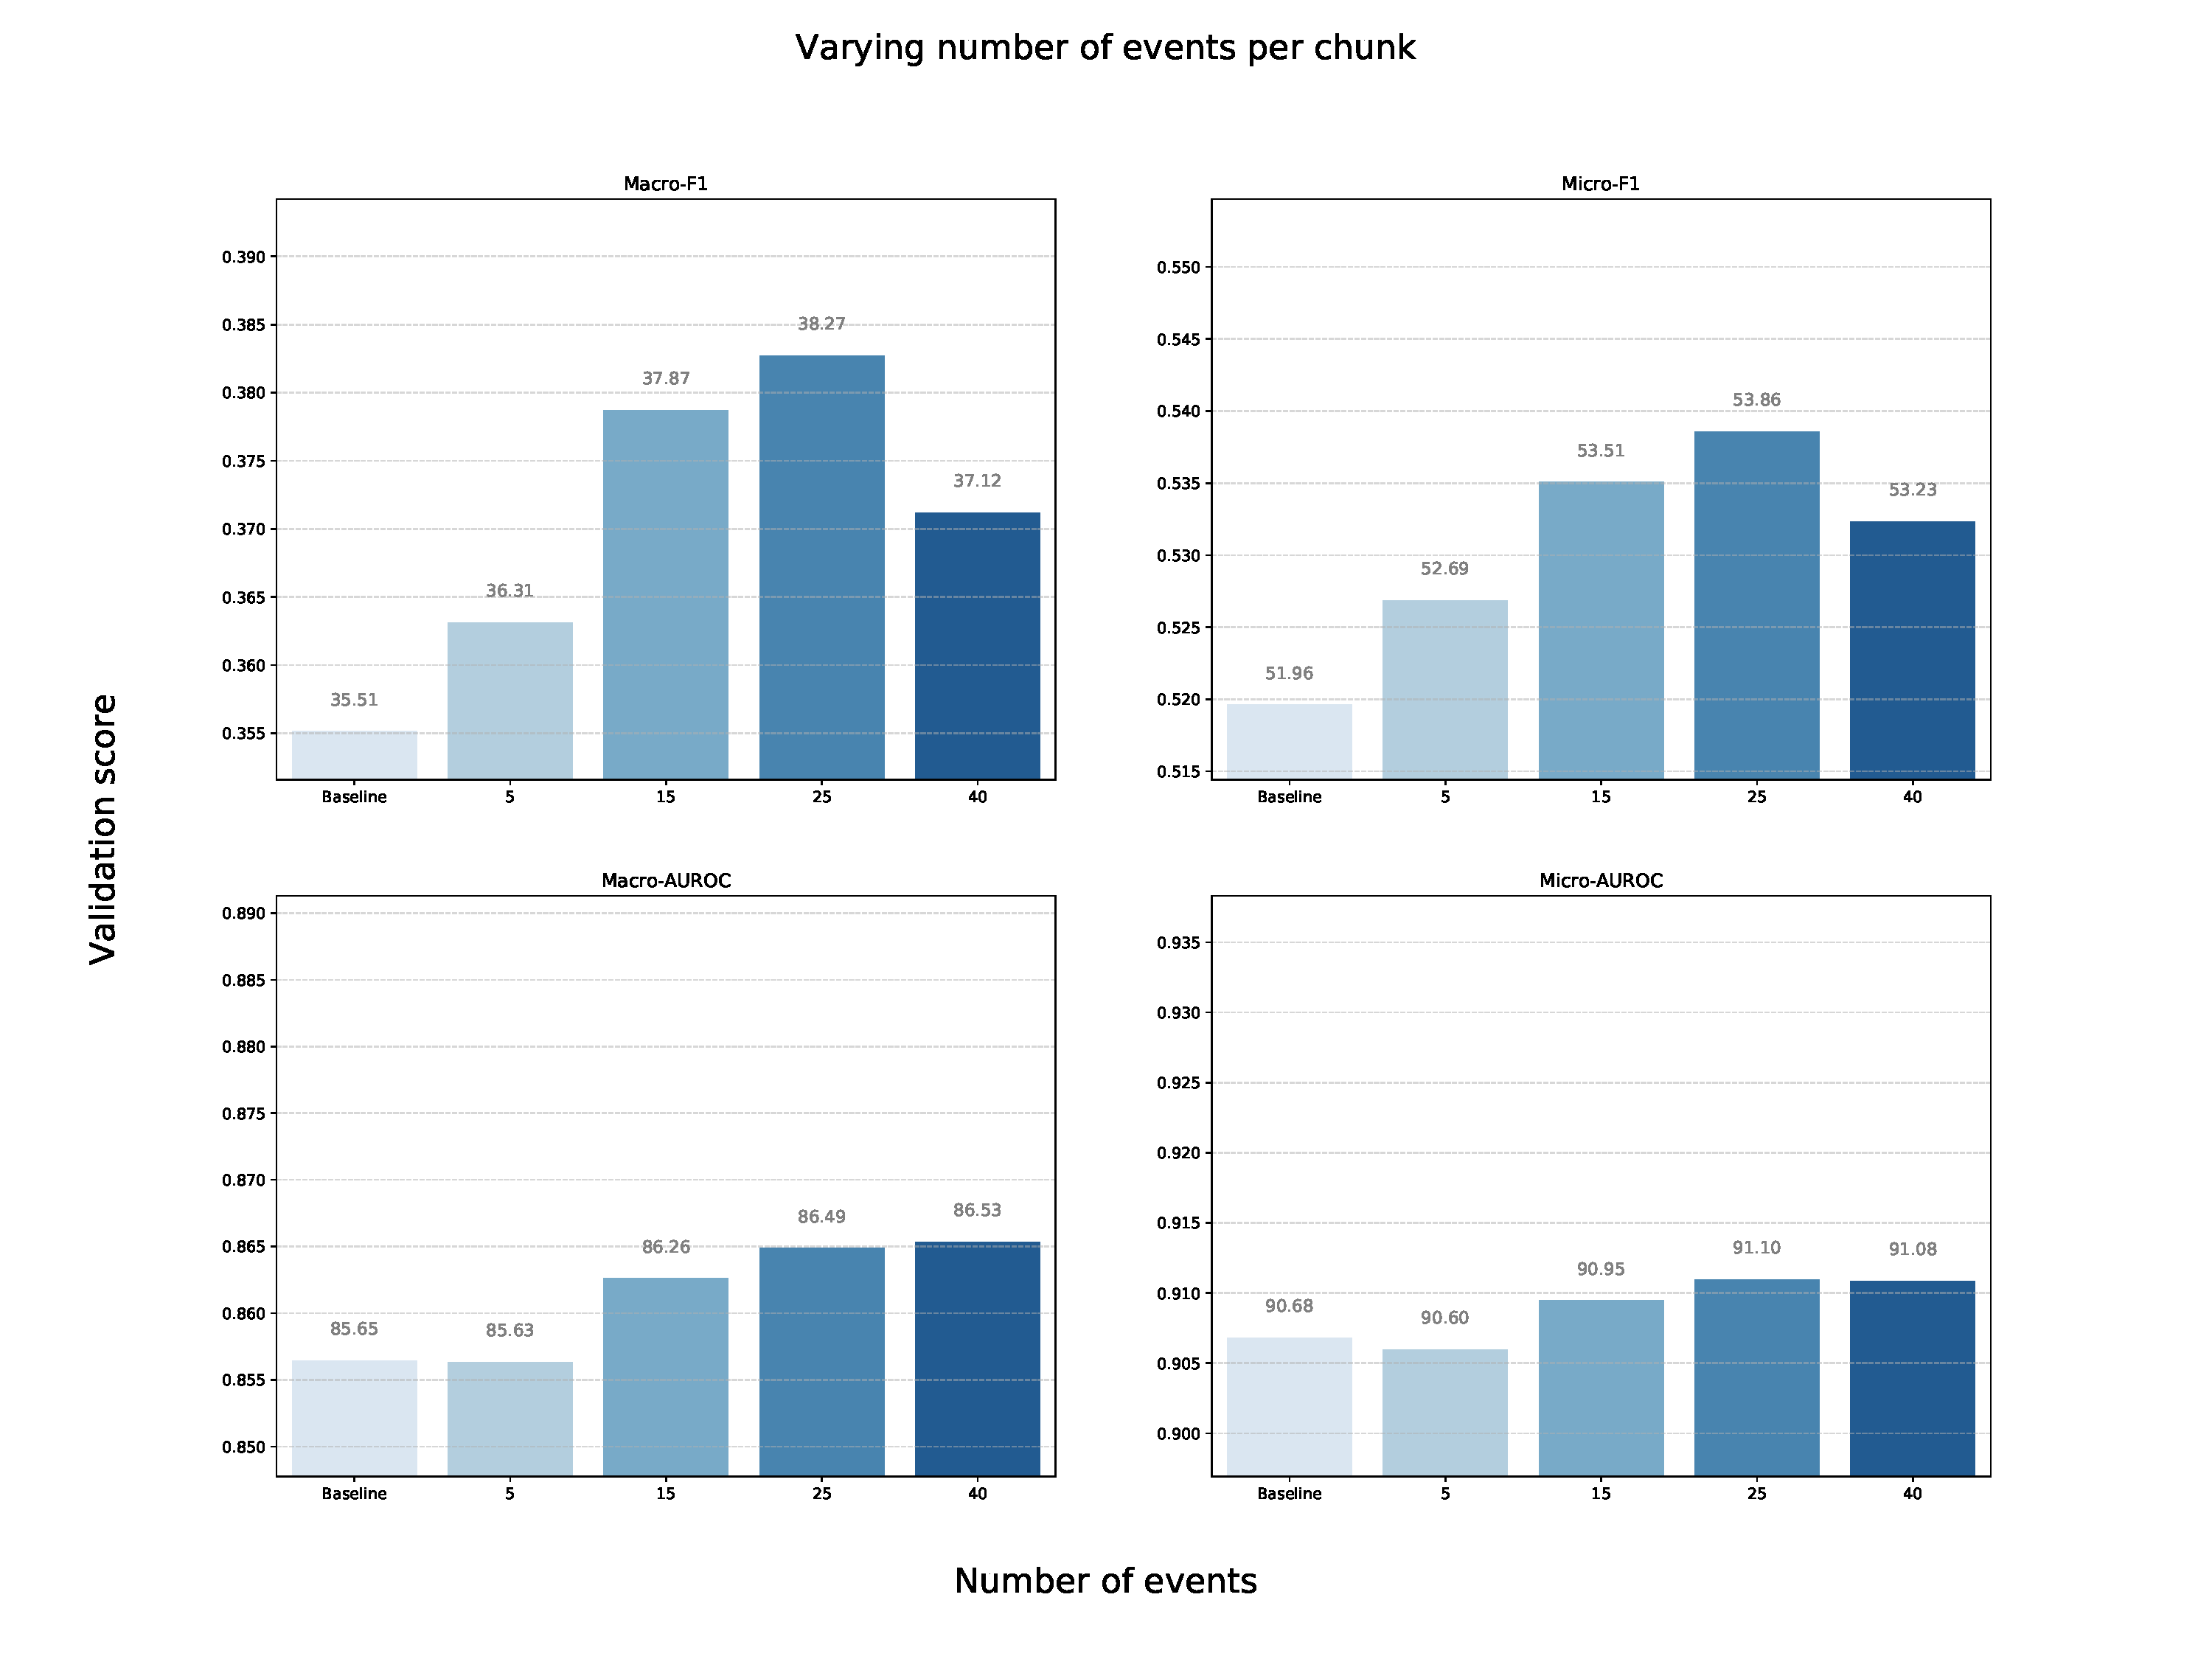
\includegraphics[width=\textwidth]{figures/exp-events.pdf}
\end{figure}
\paragraph{Discussion} As in the previous experiment, we see a clear optimum for the F1 score at 25 events per chunk and per type. Again, the conclusion is not so obvious for the AUROC score, and this metric does not seem to improve much above $K=15$.

\newpage
\subsection{Number of neighbors}
As a last experiment, we made the number of neighbors for each input entity varies. As the previous experiment, this defines the maximum number of neighbors and does not mean it will have exactly $M$ neighbors. Indeed, it is important to remember that we set a minimum \emph{WPPR} threshold of $0.0001$ that might lead to some isolated admissions having $\leq M$ neighbors.

\begin{figure}[H]
 \centering
 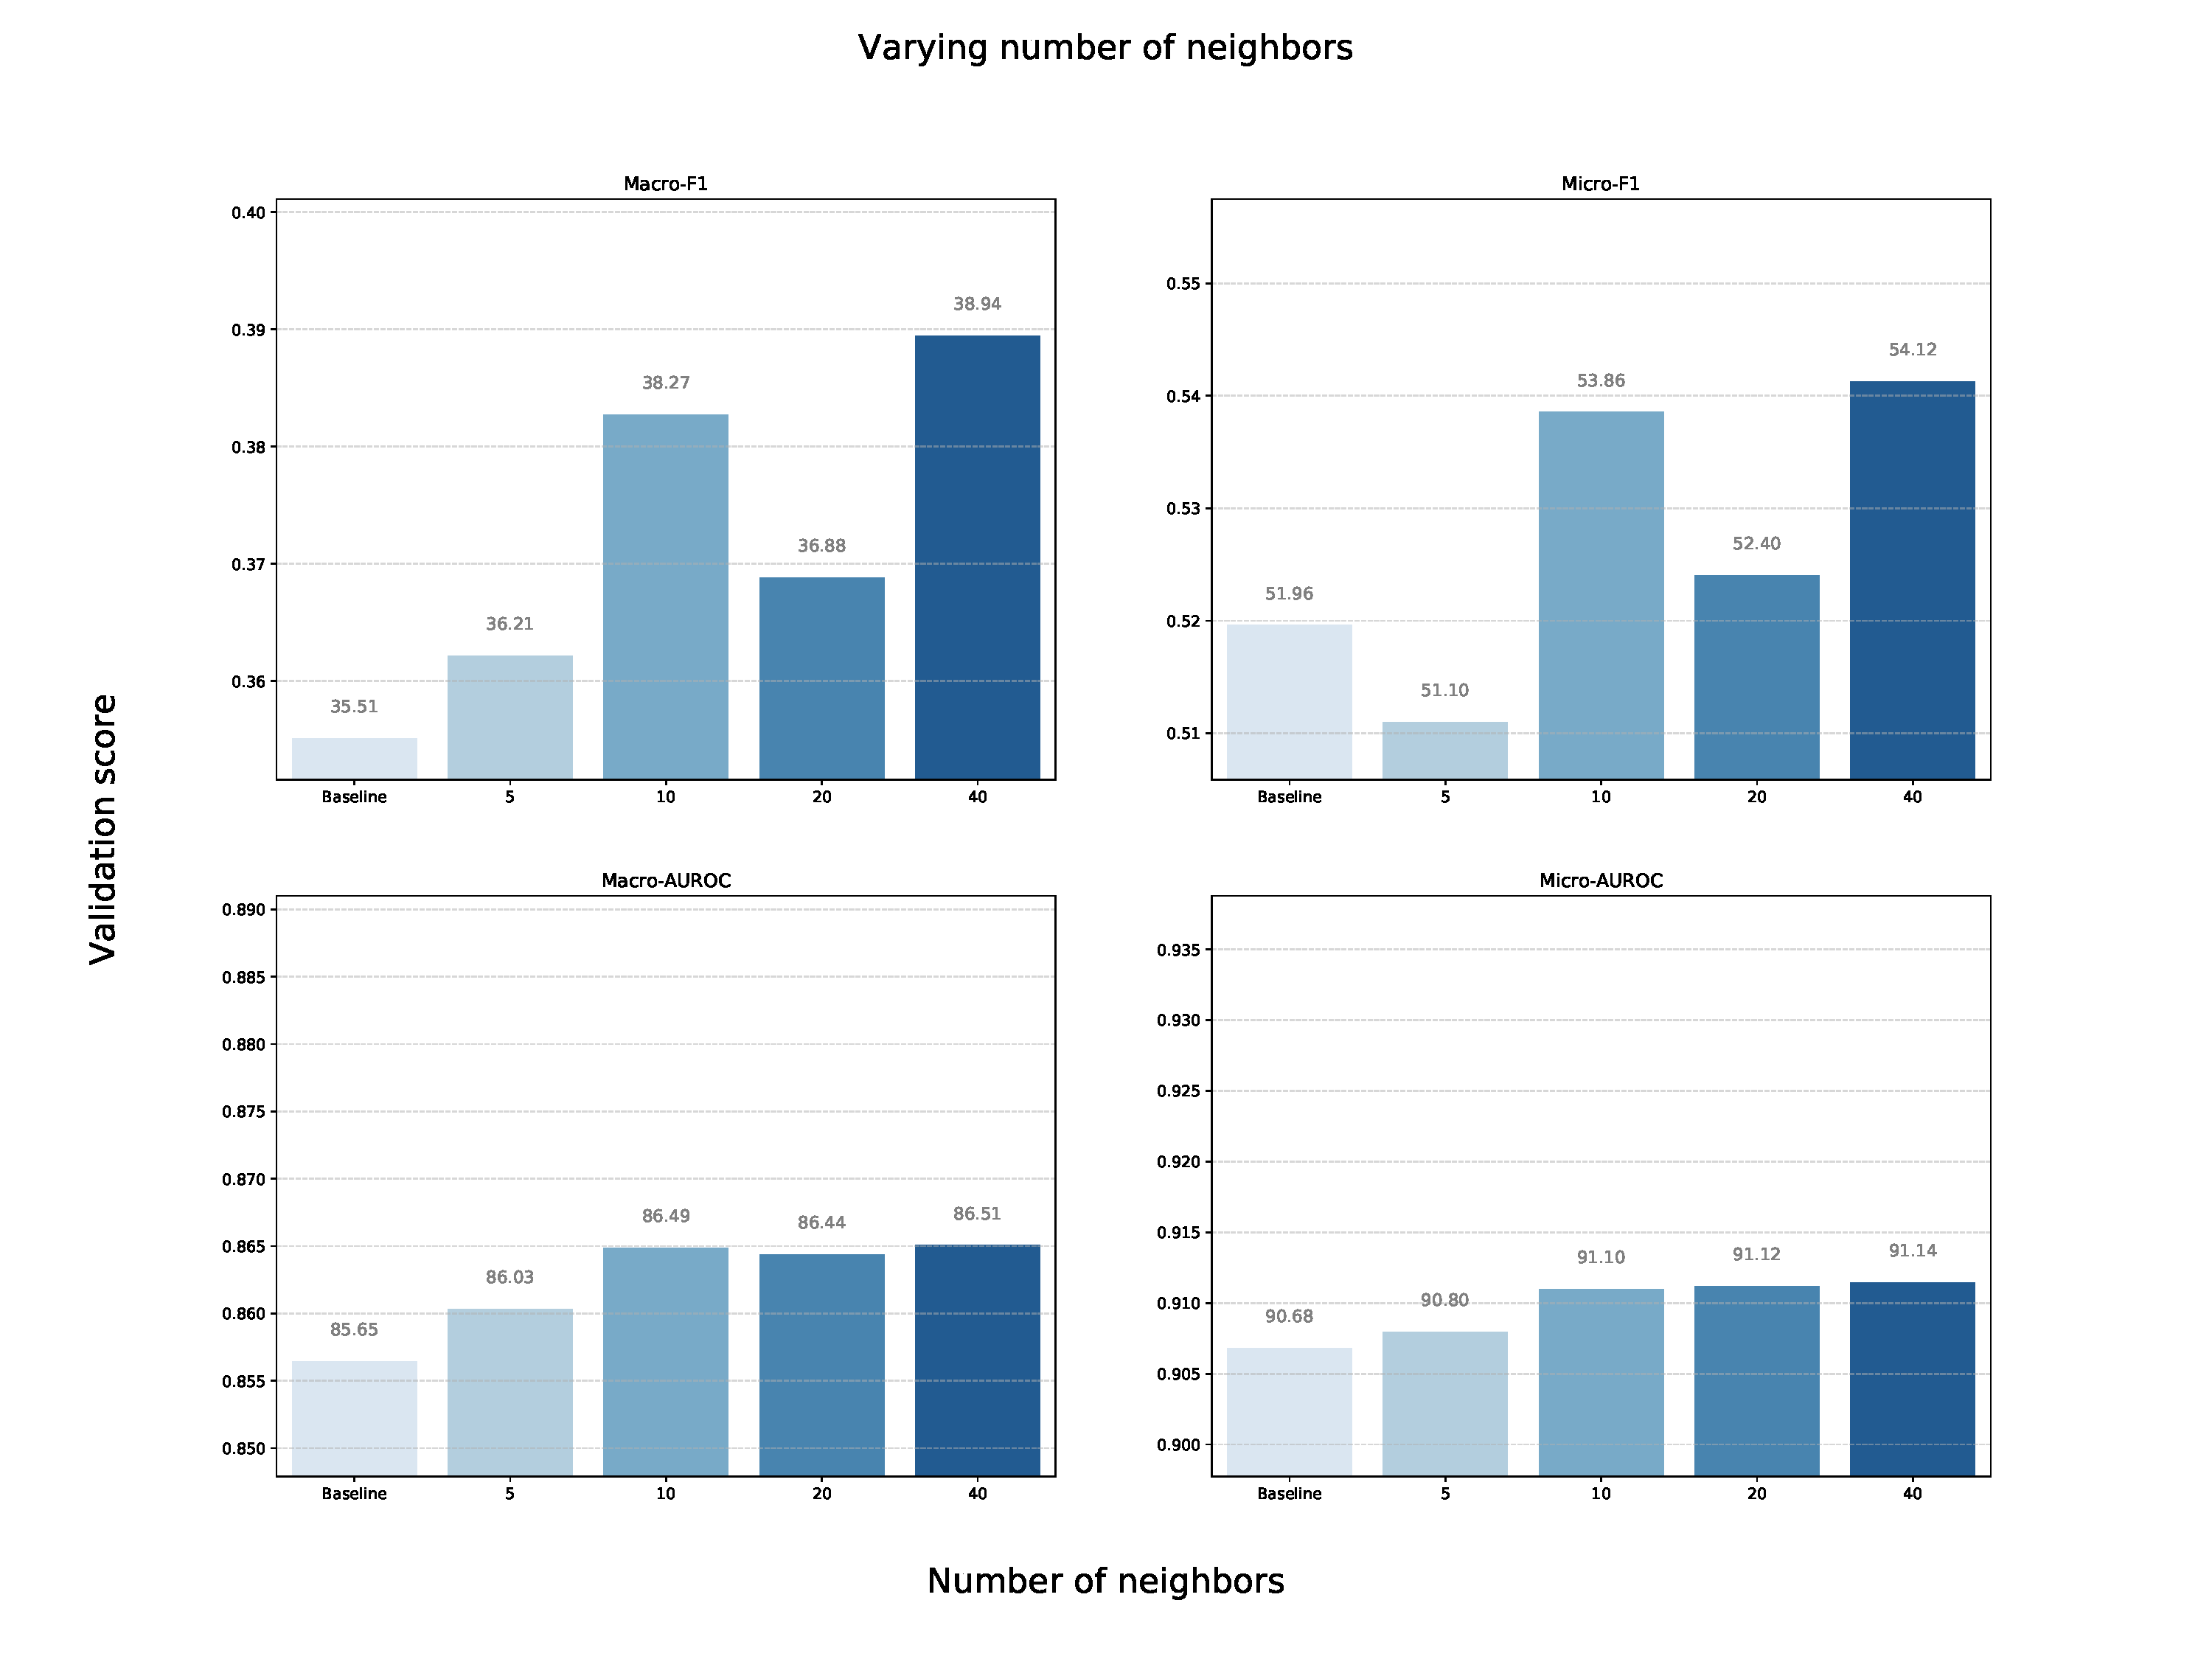
\includegraphics[width=\textwidth]{figures/exp-neighbors.pdf}
\end{figure}

\paragraph{Discussion} The results of this experiment are very interesting, yet difficult to conclude on. We can see that the number of neighbors has a huge impact on the F1 metrics, but not so much on the AUROC score. However, it is important to notice that we would expect the bar plots to have a similar shape as before. \\

That is, we would expect it to have a concave shape, where fewer neighbors means less information and thus decreased scores. Whereas, too many neighbors would add more noise than information and also hindering results. Therefore, we would expect to find an optimum value in-between but we see a drastic decrease between \textit{10} and \textit{20} neighbors, while having an increase in our metrics between \textit{20} and \textit{40} neighbors. Lastly, the scores with \textit{40} neighbors seem slightly better than with \textit{20}.

\newpage
\section{ICD9 Prediction}
\subsection{Quantitative analysis}
From these top-scoring hyper-parameters for the different groups, we selected the following parameters and ran our final evaluation for the task of predicting the top 50 ICD9 codes in a multi-class multi-classification scenario. \\

These results are all performed on the \textbf{testing set}, after all the previous hyper-parameter tuning and experiments were run on the validation set. To this end, we left the testing set untainted and the results of this section and for the task at hand will be as representative as possible from a real scenario. This testing set is made of 20\% of the dataset, totaling \textit{11'230} admissions. \\

The two following plots are interesting to compare between the baseline performances and our \emph{KG-RNN}:

\begin{figure}[H]
 \setkeys{Gin}{width=\linewidth}
 \begin{tabularx}{\textwidth}{XXXX}
  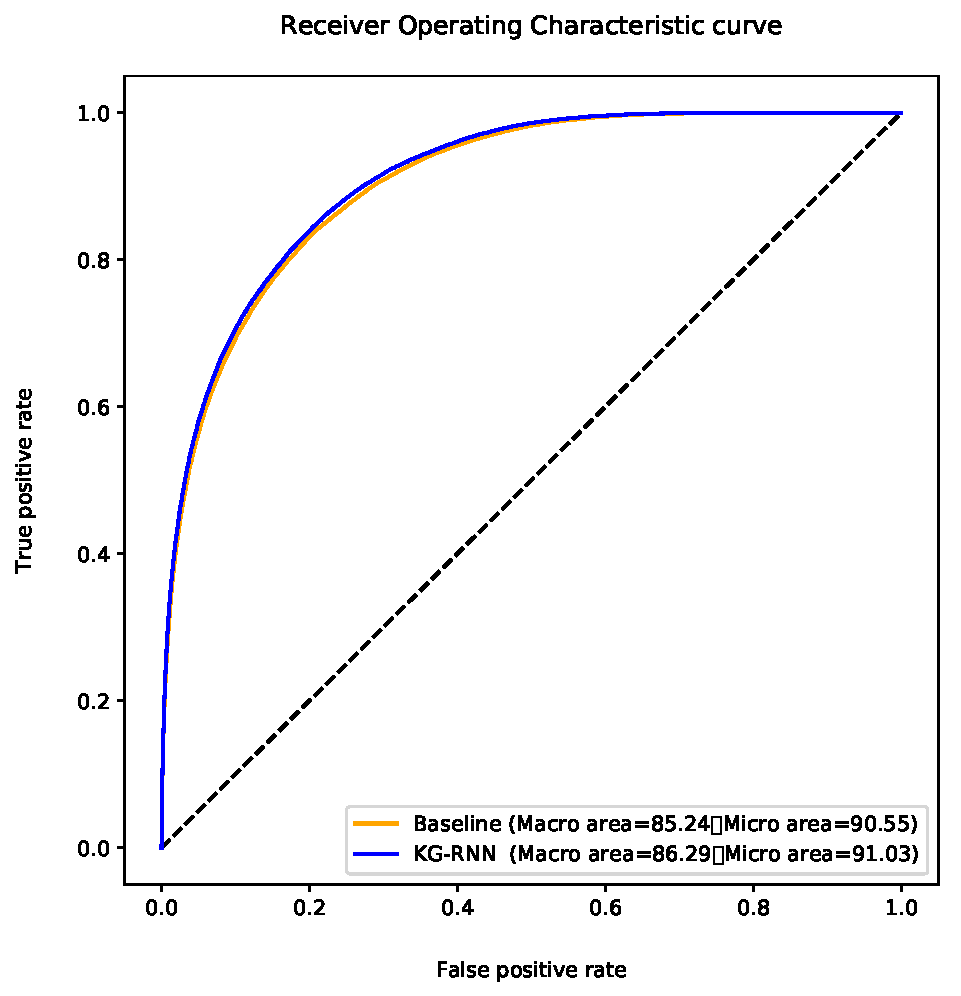
\includegraphics{figures/roc-curves.pdf} &
  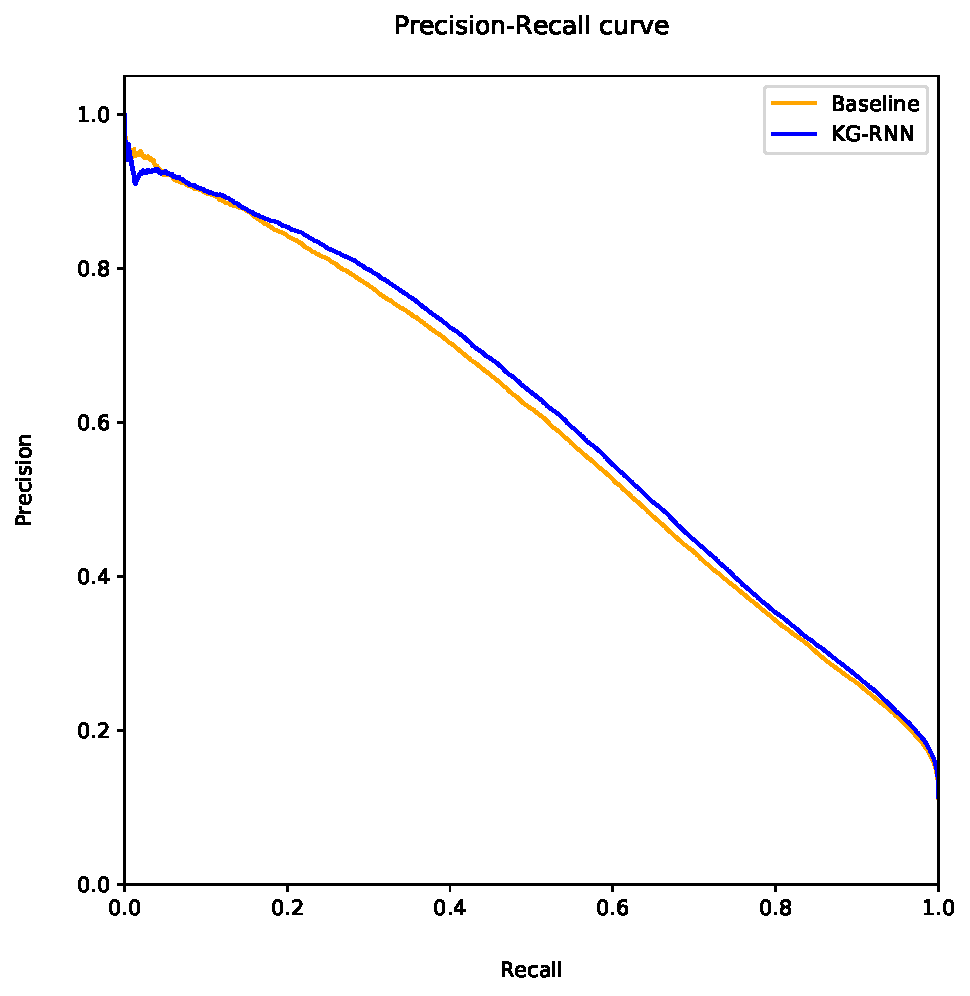
\includegraphics{figures/pr-curves.pdf}
 \end{tabularx}
 \caption{\textbf{Left}: Receiver operating characteristic curve on the testing set for both the \emph{baseline} and \emph{KG-RNN}. \textbf{Right}: Precision-recall curve on the testing set for both the \emph{baseline} and \emph{KG-RNN}.}
\end{figure}
We also evaluated the results on the different metrics that we described in the section~\ref{sec:Metrics}: \\
\begin{table}[H]
 \begin{center}
  \begin{tabular}{| p{2cm} | p{2cm} | p{2cm} | p{3cm} |}
   \hline
   &&&\\
   \textbf{Metric} & \textbf{Average} & \textbf{Model} & \textbf{Score} \\
   &&&\\ \hline
   \multirow{4}{*}{F1} & \multirow{2}{*}{Macro} & Baseline & \textbf{36.52\%} \\
   && KG-RNN & \textbf{37.90\%} (+1.38\%) \\ \cline{2-4}
   & \multirow{2}{*}{Micro} & Baseline & \textbf{51.55\%} \\
   && KG-RNN & \textbf{53.47\%} (+1.92\%) \\ \hline
   
   \multirow{4}{*}{AUROC} & \multirow{2}{*}{Macro} & Baseline & \textbf{85.24\%} \\
   && KG-RNN & \textbf{86.29\%} (+1.05\%) \\ \cline{2-4}
   & \multirow{2}{*}{Micro} & Baseline & \textbf{90.55\%} \\
   && KG-RNN & \textbf{91.03\%} (+0.48\%) \\ \hline
   
   \multirow{2}{*}{Accuracy} & \multirow{2}{*}{-} & Baseline & \textbf{92.22\%} \\
   && KG-RNN & \textbf{92.36\%} (+0.14\%) \\ \hline
  \end{tabular}
 \end{center}
\end{table}
\newpage
\paragraph{Discussion} We notice an improvement on each metric for both averages. Yet, the results are not easily distinguishable and very close to each other on the testing set compared to the validation set where the improvements from \textit{KG-RNN} were stronger. \\

To further assess the quality of our \emph{KG-RNN} model, we decided to use a statistical significance test, the McNemar's Test~\footnote{\href{https://en.wikipedia.org/wiki/McNemar\%27s\_test}{https://en.wikipedia.org/wiki/McNemar's\_test}}. Indeed, this test will allow us to get a very precise idea of the relevance of the edge that \emph{KG-RNN} seems to have over the baseline. \\

The McNemar's test requires to build a ``contingency table`` from our results, as follows: \\

\begin{table}[H]
 \begin{center}
  \begin{tabular}{ p{4cm} | p{4cm} | p{4cm} }
   & \textbf{KG-RNN is correct}  & \textbf{KG-RNN is incorrect} \\
   && \\ \hline
   && \\
   \textbf{Baseline is correct} & 510'590 (\textit{a}) & 7'247 (\textit{b}) \\
   && \\ \hline
   && \\
   \textbf{Baseline is incorrect} & 7'984 (\textit{c}) & 35'679 (\textit{d}) \\
   && \\ \hline
  \end{tabular}
 \end{center}
\end{table}

If we consider $p_b$ and $p_c$ as the theoretical cell probabilities, the null hypothesis and the alternative are:

\begin{equation*}
 \begin{aligned}
  H_0: &&p_b = p_c \\
  H_1: &&p_b \neq p_c
 \end{aligned}
\end{equation*}

In other words, \textbf{under the null hypothesis, the two models should have the same error rate.} and we can summarize this as follows:

\begin{itemize}
 \item \textbf{Fail to Reject Null Hypothesis}: Classifiers have a similar proportion of errors on the testing set.
 \item \textbf{Reject Null Hypothesis}: Classifiers have a different proportion of errors on the testing set.
\end{itemize}

Where under the null hypothesis and with a sufficient amount of data (which is our case), the statistic should follow a chi-squared distribution with 1 degree of freedom. \\

Notably, in our case the \emph{Corrected McNemar} test statistic is: \\

\begin{equation}
\chi^2 = \frac{(|b-c|-1)^2}{b+c} = \frac{(|7247-7984|-1)^2}{7247+7984} = 35.57
\end{equation}

and the associated \textbf{p-value} under $H_0$ is $P=0.0000000025$, which is extremely small and statistically significant. \\

Hence, our p-value shows sufficient evidence to reject the null in favor of the alternative hypothesis. Therefore, the two models have different performances when trained on this particular testing set, supporting the idea that the edge over the baseline is not due to randomness but rather a truly improved predictive power.

\newpage
\subsection{Qualitative Analysis}
\label{subsec:Qualitative analysis}
\paragraph{Embeddings} First off, we decided to analyze the embedding we optimized while training \emph{KG-RNN}. For this purpose, we projected our embedding matrices into two dimensions using a Uniform Manifold Approximation and Projection~\cite{2018arXivUMAP}. Then, we picked a laboratory measurement (\textbf{White Blood Cells}) and a prescription (\textbf{Sodium}) to extract their nearest neighbors in the projected 2D manifold:
\begin{multicols}{2}
 \centering
 Neighbors for \textbf{White Blood Cells}
 \begin{center}
  \begin{tabular}{| c | c |}
   \hline
   \textbf{Rank} & \textbf{Laboratory measure} \\ \hline
   1 & WBC \\ \hline
   3 & White Cells \\ \hline
   6 & Immunoglobulin A \\
   \hline
  \end{tabular}
 \end{center}\columnbreak
 \vfill
 Neighbors for \textbf{Sodium}
 \begin{center}
  \begin{tabular}{| c | c |}
   \hline
   \textbf{Rank} & \textbf{Prescription} \\ \hline
   1 & Sodium Chloride Nasal \\ \hline
   2 & Sodium Chloride 0.9\%  Flush \\ \hline
   5 & Famotidine \\
   \hline
  \end{tabular}
 \end{center}
\end{multicols}

In the first case (i.e. \textit{White Blood Cells}), it is very interesting to notice that among the neighbors, we first find an abbreviation of the same laboratory measurement: \textbf{WBC}, as well as a short name of it at the third-closest neighbor: \textbf{White Cells}. Finally, we also see the compelling evidence that the embedding is of good quality by the positioning of \textbf{Immunoglobulin A}, which are antibodies produced by white blood cells. \\

In the second table, we see that \textit{Sodium} is close to its related prescriptions in the first two nearest neighbors. Whereas, \textbf{Famotidine} is also ranked very close at the fifth rank, and it is known in the medical field that Famotidine is often given in \textbf{0.9\% Sodium Chloride} through intravenous, our second neighbor. \\

Overall, we can see with these two examples that \emph{KG-RNN} has not only learned similar events, such as ``White Blood Cells`` and ``WBC``, but also intrinsically and correlated linked events. Indeed, as we noticed, our deep learning architecture mapped events close to each other in the embedding space if they are related in the medical domain, learning more complex interactions.

\newpage
\paragraph{Predictions} Secondly, to have a better understanding of the value provided by \emph{KG-RNN} over the baseline, we extracted a few samples where the baseline was incorrect but KG-RNN was right in its prediction (represented by \textit{c} in the ``contingency table``). \\

From the extracted samples and to the purpose of understanding the differences, we also checked the information conveyed by neighbors of the input admission. To this end, we are able to analyze and visualize where the correctness of \emph{KG-RNN} over the baseline comes from. \\

In the following graphs, the first row corresponds to the input admission while the other ones to its neighbors. Each red line shows an ICD9 code actually diagnosed at discharge (i.e. the ground truth), and the horizontal gray line represents the default 0.5 threshold above which a prediction is considered.  In the input admission graph (first row), the orange and blue bars are the estimated probabilities by the models, respectively the baseline and \emph{KG-RNN}. Finally, in the neighbor rows, the dark-gray bars represent their final diagnoses (i.e. entity static information) as one-hot vectors. \\

\begin{figure}[H]
 \centering
 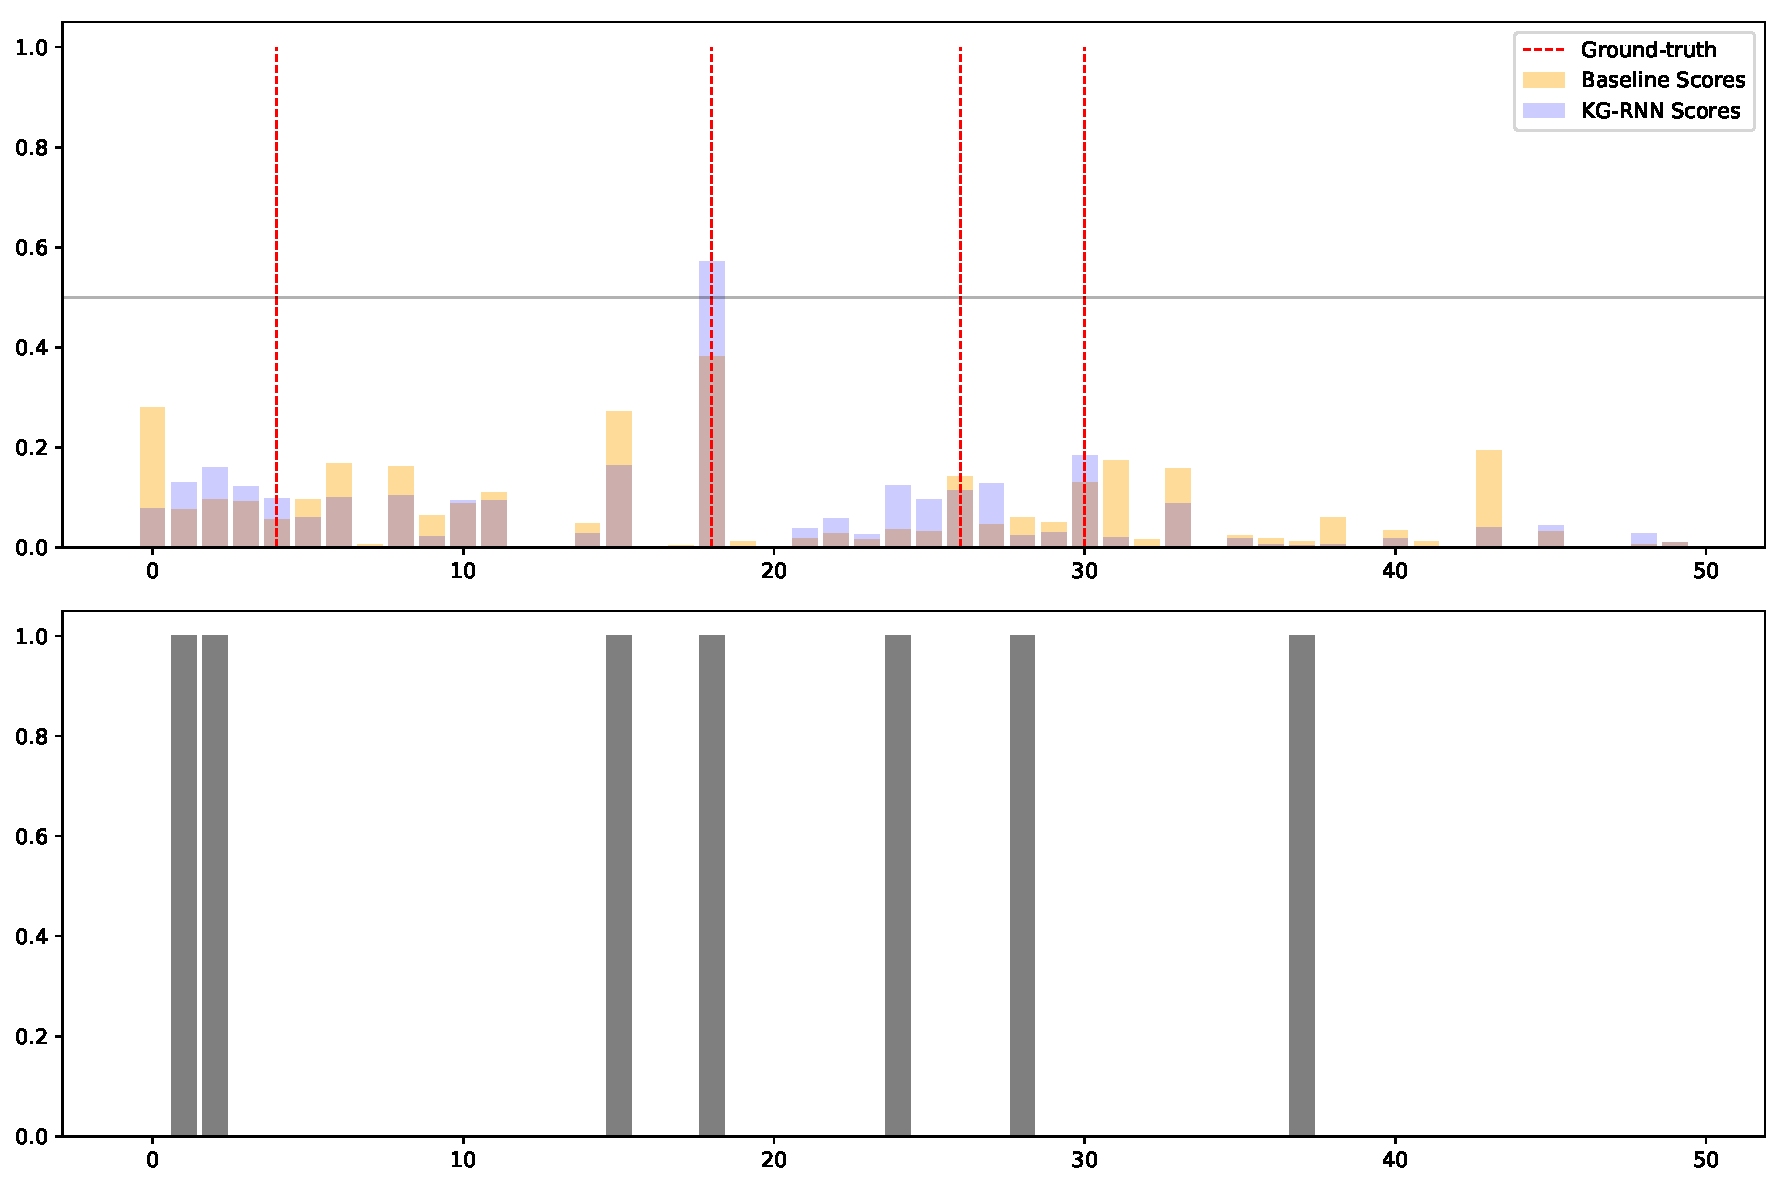
\includegraphics[width=0.8\textwidth]{figures/preds-0.pdf}
 \caption{In this plot we can see that the neighbors provide the necessary information to \emph{KG-RNN} to improve over the baseline. Indeed, this model does not detect any diagnostic, whereas KG-RNN is able to predict the second one with the help of its neighbor. Namely, we hypothesize that since its neighbor static information conveys the ICD9 code of interest (the second one), it helped pushing the confidence of KG-RNN upward, above the 0.5 decision threshold.}
\end{figure}

\newpage
The ICD9 codes of the ground truth and the neighbor from the previous figure are summarized in the following table:

\begin{table}[H]
 \begin{center}
  \textbf{Input admission} \\
  
  \begin{tabular}{| c | c | p{8cm} |}
   \hline
   \textbf{Rank} & \textbf{ICD9 Code} & \textbf{Description} \\ \hline
   4 & 272.4 & Other and unspecified hyperlipidemia  \\ \hline
   18 & 401.9 & Unspecified essential hypertension \\ \hline
   26 & 486 & Pneumonia, organism unspecified \\ \hline
   30 & 530.81 & Esophageal reflux \\ \hline
  \end{tabular}
 \end{center}
\end{table}
\begin{table}[H]
 \begin{center}
  \textbf{Neighbor} \\
  
  \begin{tabular}{| c | c | p{8cm} |}
   \hline
   \textbf{Rank} & \textbf{ICD9 Code} & \textbf{Description} \\ \hline
   1 & 244.9 & Unspecified acquired hypothyroidism \\ \hline
   2 & 250.00 & Diabetes mellitus without mention of complication, type II or unspecified type, not stated as uncontrolled \\ \hline
   15 & 38.93 & Unspecified septicemia \\ \hline
   18 & 401.9 & Unspecified essential hypertension \\ \hline
   24 & 427.31 & Atrial fibrillation \\ \hline
   28 & 507.0 & Pneumonitis due to inhalation of food or vomitus \\ \hline
   37 & 96.6 & Late syphilis, latent \\ \hline
  \end{tabular}
 \end{center}
\end{table}

It is interesting to see that even if the neighbor diagnoses do not match the ground truth \textit{perfectly}, some ICD9 codes still convey information for the input admission. Indeed, if we look at the number \textbf{26} in the input admission (i.e. \textit{Pneumonia}), it could be linked to the number \textbf{28} of the neighbor (i.e. \textit{Pneumonitis}). However, even if the final diagnoses are different (``Pneumonitis`` indicates inflammation of lung tissues, whereas ``Pneumonia`` is inflammation caused by an infection), the admissions are linked through their pre-diagnosis and thus one may carry information on the other. \\

Therefore, using the ICD9 code hierarchy may help the model to make sense from neighbors diagnoses and increase predictive power for the input admission. This potential trail is further described in the appropriate section~\ref{sec:Future Work} of the last chapter.

\newpage
\begin{figure}[H]
 \centering
 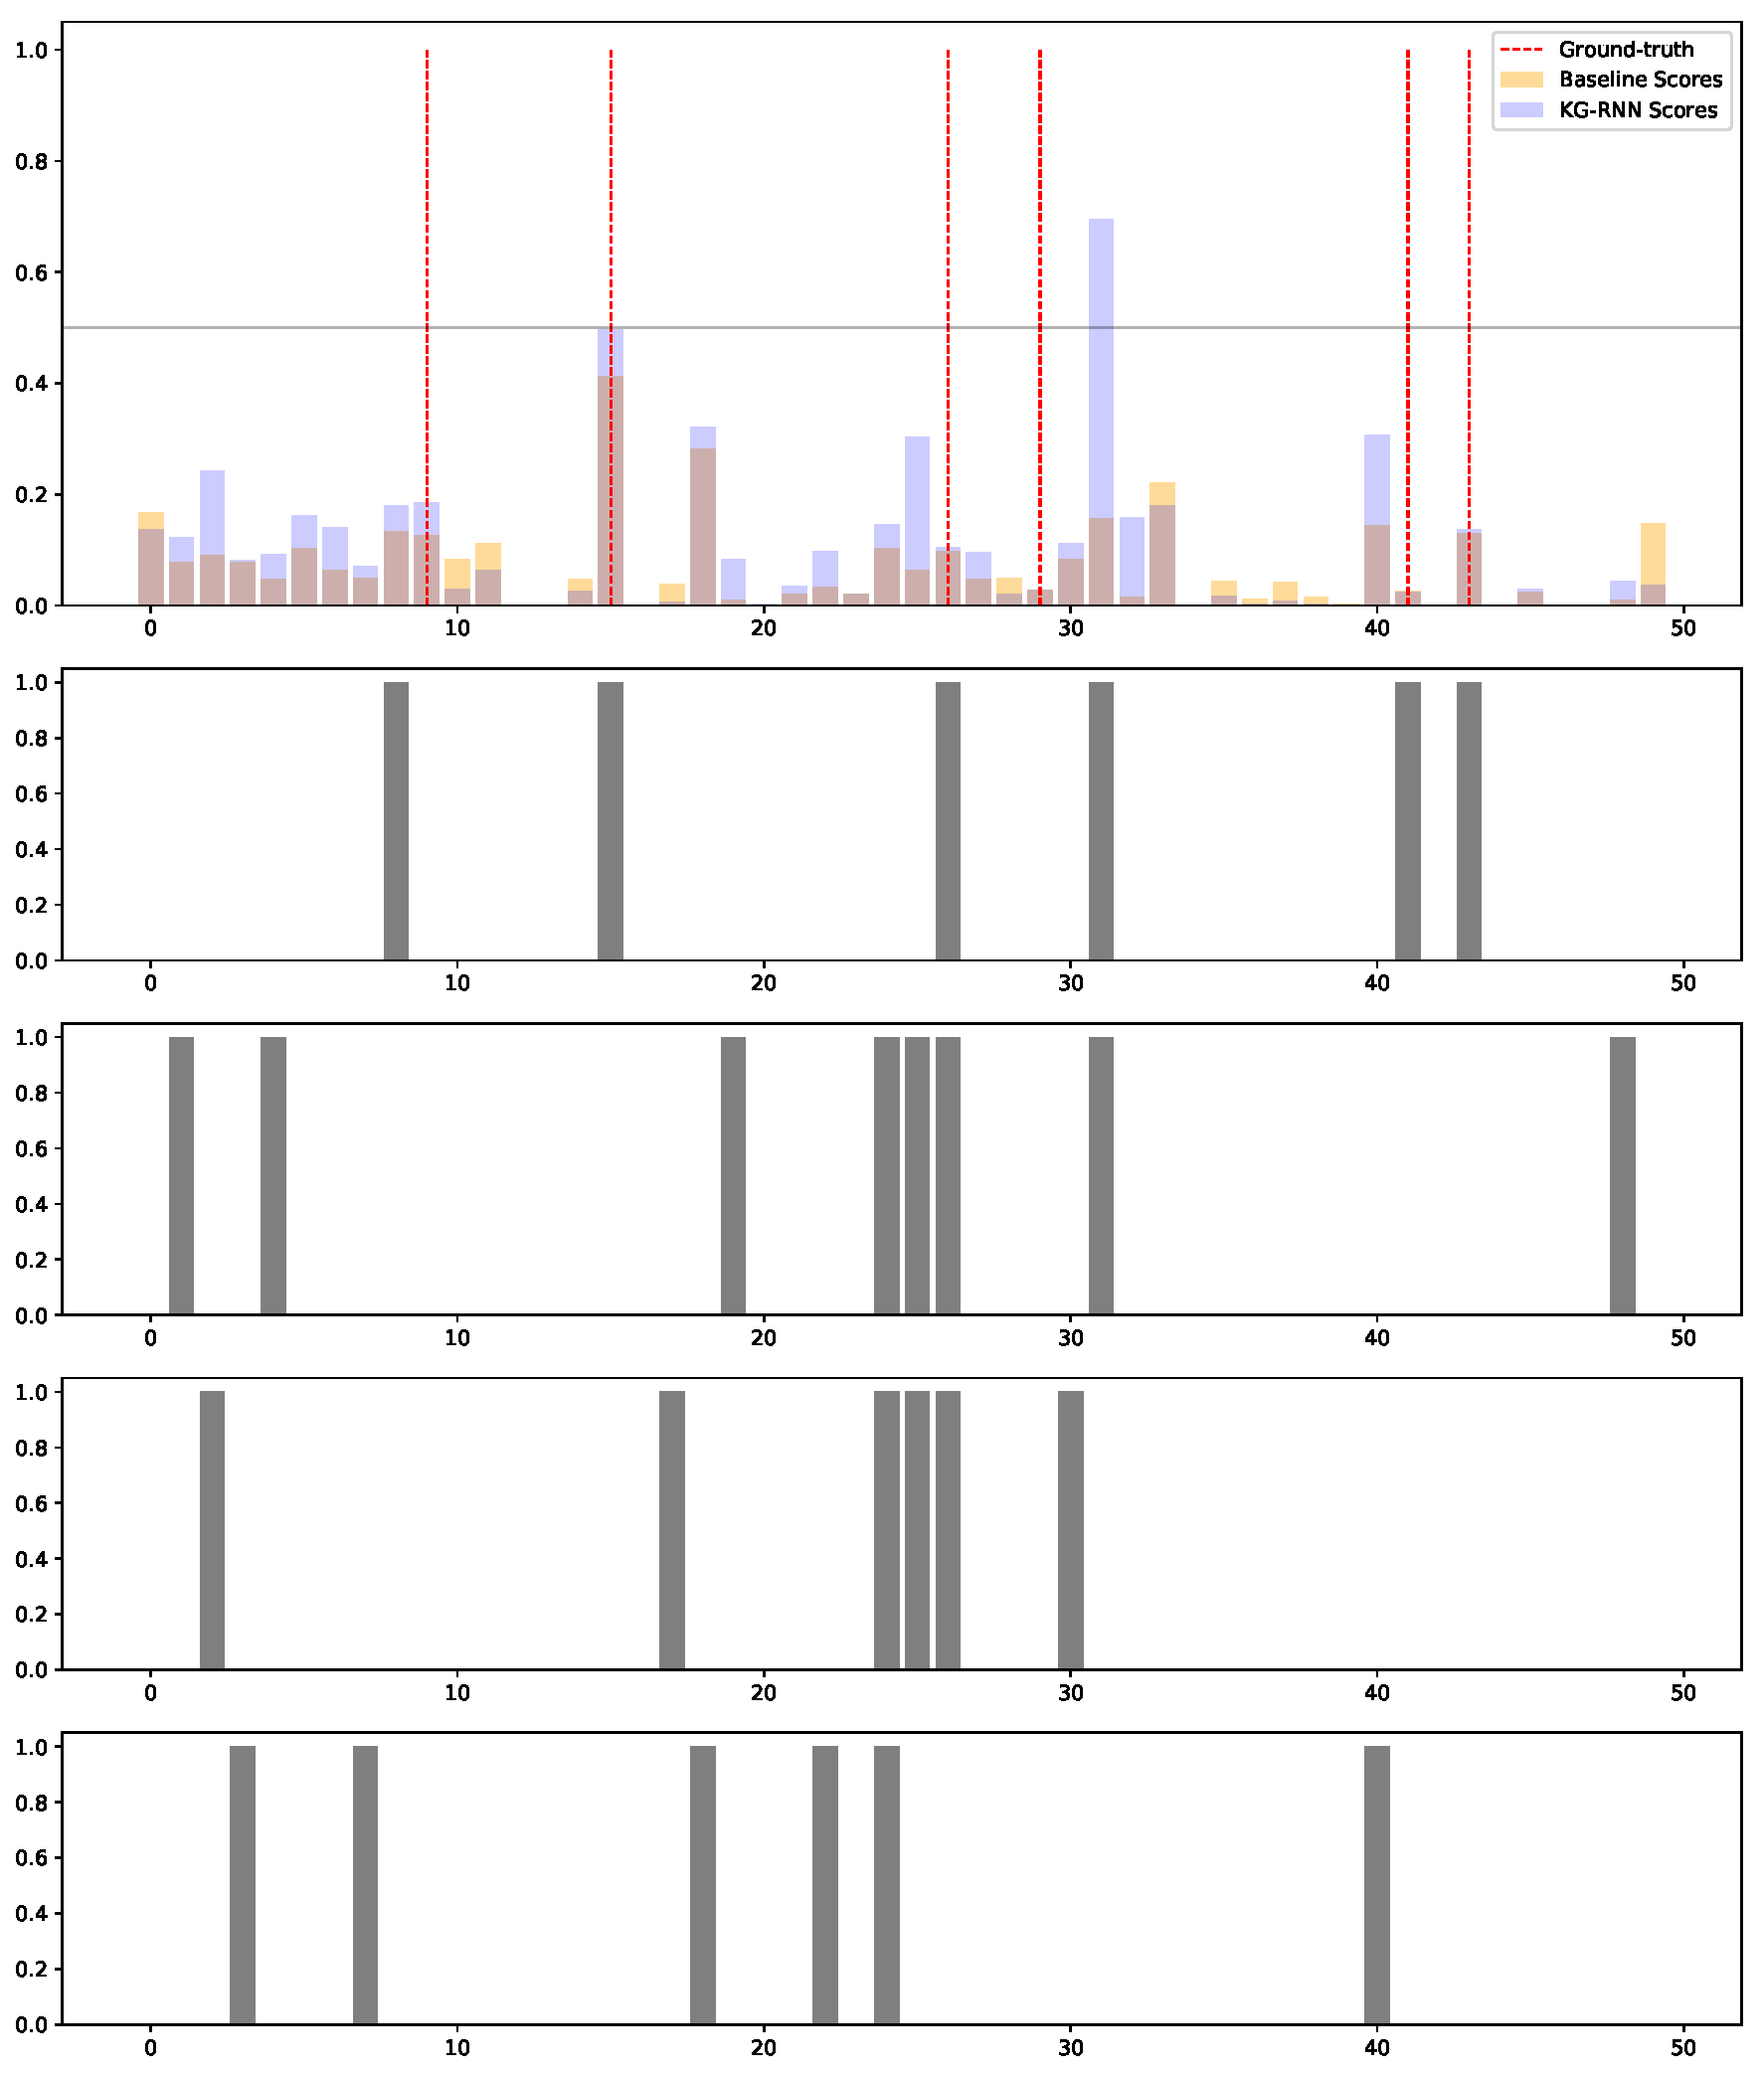
\includegraphics[width=0.8\textwidth]{figures/preds-1.pdf}
 \caption{In this plot, the input admission has 4 neighbors with different final diagnoses (static information), and we also notice interesting behavior of \emph{KG-RNN} compared to the baseline. In this scenario, we see that the first neighbor helps pushing the confidence of the model over the decision threshold for the second diagnosed ICD9 code. However, we also see that \emph{KG-RNN} is misled by the first two neighbors that are wrongly pushing ICD9 number thirty-one over the decision threshold. This highlights the importance of a good knowledge graph construction and neighbors extraction algorithm.}
\end{figure}

To conclude, we see that neighbors are having a big impact on KG-RNN, as the predictions where $\mbox{Score}_{\mbox{baseline}} \ge \mbox{Score}_{\mbox{KG-RNN}}$ occur when none of the neighbors have a matching ICD9 code. On the other hand, when one or more of the neighbors have a certain ICD9 code, the corresponding score for \emph{KG-RNN} on the input admission is consistently pushed upwards. This reveals how much KG-RNN learns to rely on its neighbors to score its predictions.